\section{Evaluation}
\label{sec:evaluation}

We evaluate \sysname across the four contributions claimed in
\S~\ref{sec:introduction}: (i) unlearning effectiveness under three
approximate methods plus an exact-retraining baseline (E6), (ii)
on-chain cost on PureChain versus Polygon Amoy (E7), (iii)
scalability of round validation up to $N\!=\!500$ participants (E8),
and (iv) utility recovery through the revocation event. Two short
on-chain demos additionally validate Properties~\ref{prop:liveness}
and~\ref{prop:verifiability}. The complete reproducibility recipe
lives in supplementary \texttt{docs/eval-protocol.md}.

\subsection{Experimental setup}
\label{sec:eval-setup}

The primary federation is a 9-client N-BaIoT autoencoder anomaly
detector~\cite{meidan2018nbaiot}, one client per IoT device (doorbells,
thermostats, baby monitors, security cameras, webcams). Each client
holds 5{,}000 benign-traffic rows over 115 network features; the
global model is a symmetric MLP autoencoder
($115\!\to\!75\!\to\!50\!\to\!25\!\to\!10$, ReLU, dropout 0.1) trained
with FedAvg over 30 rounds (Flower framework~\cite{beutel2020flower}),
batch size 256, learning rate $10^{-3}$, random seed 42. At round 30 we simulate a GDPR Art.~17 erasure event
against client 5 (\textit{Provision\_PT\_838\_Security\_Camera}) and
trigger one of three approximate unlearning methods (SISA-Fed,
gradient ascent, FedEraser) or, as the exact reference, full
retraining of an 8-client federation from scratch. All experiments
record an environment fingerprint (commit hash, library versions,
hardware, seed) in an \texttt{env.json} alongside the metric JSON.

On-chain experiments run against the live contracts deployed on both
PureChain (chainId \texttt{900520900520}, gas-free, PoA$^2$) and
Polygon Amoy (chainId \texttt{80002}, gas-based, PoS). The verifier
set $\mathit{VC}$ is five ECDSA keys with threshold $t = 3$;
$\dmax = 1000$ blocks unless otherwise noted.

\subsection{Unlearning effectiveness}
\label{sec:eval-unlearning}

Table~\ref{tab:t1} reports each method's three independent MIA
scores against the revoked client's member set. The on-chain
\texttt{submitAttestation} predicate (Eq.~\ref{eq:accept}) accepts a
UA iff all three scores sit below $\tauMIA\!=\!0.55$.

\begin{table}[t]
\centering
\caption{Table 1 --- Unlearning effectiveness (E6). MIA scores
against the revoked client's training data, evaluated on the
post-unlearning model. The on-chain gate accepts a UA iff all
three are below $\tauMIA = 0.55$.}
\label{tab:t1}
\footnotesize
\setlength{\tabcolsep}{4pt}
\resizebox{\columnwidth}{!}{% Table 1 — Unlearning effectiveness (MIA scores)
% generated by fl/experiments/collect_results.py
\begin{tabular}{lcccc}
\toprule
Method & Shadow MIA & LiRA & Label-only & On-chain accept \\
\midrule
No unlearning (baseline) & 0.5455 & 0.5000 & 0.0060 & \checkmark \\
Gradient ascent & 0.4380 & 0.5000 & 0.0030 & \checkmark \\
SISA-Fed & 0.2542 & 0.5000 & 0.0862 & \checkmark \\
FedEraser & 0.5232 & 0.5000 & 0.0050 & \checkmark \\
Naive retrain (exact ref.) & 0.5843 & 0.5000 & 0.0138 & $\times$ \\
\bottomrule
\end{tabular}
}
\end{table}

Three observations stand out. \textbf{First,} all three approximate
unlearning methods produce UAs the chain accepts: shadow scores
fall to $0.438$ (gradient ascent), $0.254$ (SISA-Fed), and $0.523$
(FedEraser); LiRA and label-only scores remain well below
$\tauMIA$. \textbf{Second}, the naive-retrain baseline ---
a model trained from scratch that has \emph{never seen} client 5's data
--- yields a shadow score of $0.584$, \emph{above} $\tauMIA$, and is
rejected by the same on-chain gate. The shadow MIA picks up client
5's distinctive network-traffic distribution rather than true
membership, a known confound of shadow-model
attacks~\cite{shokri2017mia} on distribution-shifted data; LiRA and
the label-only attack, both more sensitive to specific membership
than to distribution, score $0.500$ and $0.014$ respectively on the
same model. The protocol behaves correctly throughout --- it is
faithful to MIA evidence, not to the data controller's claim
--- and \S~\ref{sec:discussion} treats the asymmetry as an
MIA-selection result rather than a protocol bug. \textbf{Third}, gradient ascent's
shadow score ($0.438$) is \emph{lower} than naive retrain's ($0.584$):
actively anti-fitting the revoked data moves the model further from
client 5's distribution than a model that never saw it. The three
approximate methods thus trace out a forgetting-versus-utility Pareto
frontier --- SISA-Fed at the strong-forgetting end, gradient ascent
and FedEraser at the preserve-utility end --- which the utility
recovery curves (\S~\ref{sec:eval-utility}) make explicit.

End-to-end on-chain attestation of all three approximate methods
executed against PureChain. The transitionToUnlearned hook fired in
the same transaction as
\texttt{submitAttestation}; final
$\mathit{CR}.\mathtt{stateOf}$ returned \textsc{Unlearned} (state 5)
for each token. Representative gradient-ascent PureChain tx hashes
(prefixes of full 32-byte values): updateModelHash
\texttt{0x6e3b\ldots a0b8}, grantConsent
\texttt{0x92af\ldots 4be3}, revokeConsent
\texttt{0xf005\ldots d3fb}, submitAttestation
\texttt{0x7910\ldots 4a39}; per-method tx records in supplementary
\texttt{onchain\_attestation.json}.

\subsection{Gas cost comparison}
\label{sec:eval-gas}

Table~\ref{tab:t2} reports per-operation gas usage and the
corresponding cost on each chain, taken from a lifecycle ×10
variance run (E7). USD figures use POL/USD = $0.095347$ fetched
from CoinGecko on the measurement day; raw gas counts and Wei
costs are deterministic and chain-state-dependent.

\begin{table}[t]
\centering
\caption{Table 2 --- Per-operation gas and cost (E7), lifecycle ×10
mean. PureChain costs are exactly $\$0$; Amoy costs are non-zero.
Per-DS lifecycle = sum of the four ops.}
\label{tab:t2}
\footnotesize
\setlength{\tabcolsep}{3pt}
\resizebox{\columnwidth}{!}{% Table 2 — Per-operation gas + USD (lifecycle ×10 means)
% generated by fl/experiments/collect_results.py
\begin{tabular}{lrrrr}
\toprule
Operation & PureChain gas & Amoy gas & Amoy MATIC & Amoy USD \\
\midrule
\texttt{updateModelHash} & 30,074 & 32,673 & 0.0010 & \$0.00009 \\
\texttt{grantConsent} & 144,868 & 153,568 & 0.0046 & \$0.00044 \\
\texttt{revokeConsent} & 107,904 & 96,404 & 0.0029 & \$0.00028 \\
\texttt{submitAttestation} (3-of-5) & 102,903 & 137,600 & 0.0041 & \$0.00039 \\
\midrule
\textbf{Per-DS lifecycle} & \textbf{385,750} & \textbf{420,245} & \textbf{0.0126} & \textbf{\$0.00120} \\
\bottomrule
\end{tabular}
}
\end{table}

Per-data-subject lifecycle cost is $\$0$ on PureChain and $\$0.00120$
on Amoy. Gas usage differs by up to $34\%$ between the two chains
(\texttt{submitAttestation}: $102{,}903$ on PureChain versus
$137{,}600$ on Amoy) due to opcode-pricing differences between the
PoA$^2$ schedule and Polygon's EIP-2929-equipped schedule; the
dominant cost factor at scale is the gas price (zero versus
$\sim\!30$ gwei), not the gas count. \S~\ref{sec:eval-scalability}
quantifies the recurring per-FL-round cost as deployments grow.

\subsection{Scalability of round validation}
\label{sec:eval-scalability}

Figure~\ref{fig:f1} reports gas usage and equivalent USD cost for
$\texttt{validateRound}(N)$ as $N$ scales from 5 to 500 participants.
On PureChain the full sweep ran live; on Amoy only $N \in \{5, 10\}$
were measured directly (wallet-budget constraint) and the remaining
points are extrapolated via least-squares linear fit
$\mathrm{gas}(N) \approx 40{,}002 + 12{,}202 N$, which the
PureChain measurements (slope $7{,}616$) confirm as exactly linear
($R^2 \!\approx\! 1$).

\begin{figure}[t]
\centering
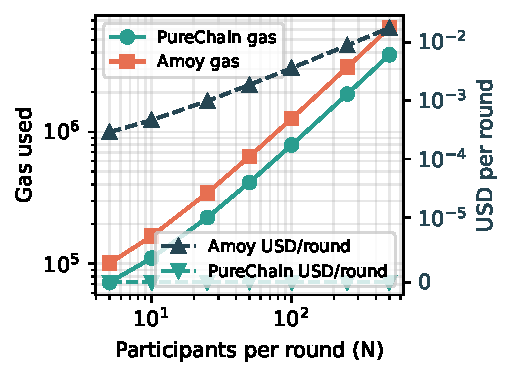
\includegraphics[width=0.92\columnwidth]{figures/figure1_scalability.pdf}
\caption{Figure 1 --- Scalability of $\texttt{validateRound}(N)$
(E8). Solid lines: live gas measurements. Dashed lines: per-round
USD cost. PureChain cost line is at zero across all $N$; Amoy
projects to $\$0.0176$ at $N\!=\!500$.}
\label{fig:f1}
\end{figure}

PureChain's per-participant slope is $\sim\!38\%$ lower than Amoy's
--- the EIP-2929 cold-SLOAD pricing ($2{,}100$ gas) dominates the
linear term on Amoy. The cost story is dominated by gas \emph{price}:
on Amoy a single $N\!=\!500$ round-validation costs $\$0.0176$; on
PureChain the same operation costs $\$0$. Combined with a typical
100-FL-rounds-per-day cadence, Amoy accumulates $\$1.76$/day per
deployment; 10 concurrent deployments would cost $\sim\!\$17.57$/day
on Amoy and $\$0$ on PureChain. Gas-free infrastructure is not an
optimisation; it is a different cost class.

\subsection{Utility recovery after revocation}
\label{sec:eval-utility}

Figure~\ref{fig:f2} plots the size-weighted central reconstruction
error for five trajectories diverging at round 30, the revocation
point. The baseline 9-client federation continues to round 40 with
all clients; the other four trajectories drop client 5 and resume
FL for ten further rounds, each starting from a different round-30
checkpoint.

\begin{figure}[t]
\centering
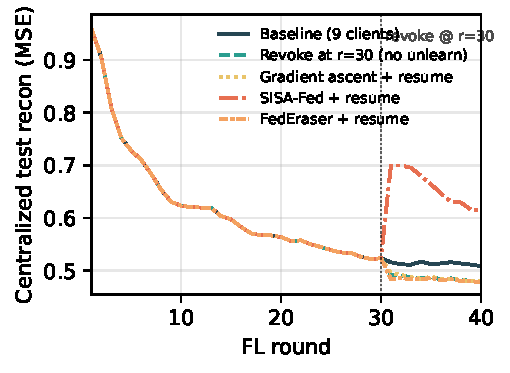
\includegraphics[width=0.92\columnwidth]{figures/figure2_utility_recovery.pdf}
\caption{Figure 2 --- Utility recovery (E6). Centralized test
reconstruction error per FL round. The four post-revocation
trajectories diverge at round 30; SISA-Fed pays a real utility cost,
gradient ascent and FedEraser converge to within $0.2\%$ of plain
post-revoke by round 40.}
\label{fig:f2}
\end{figure}

The post-revoke trajectory (no unlearning step) ends at $0.4796$
test reconstruction error, $5.7\%$ \emph{better} than the
9-client baseline ($0.5087$): client 5 was an outlier in the benign
traffic distribution and its removal lets the federation fit the
remaining devices more tightly. Gradient ascent and FedEraser end at
$0.4794$ and $0.4783$ respectively --- the unlearning step is
free of utility cost in both cases. SISA-Fed is the outlier: its
round-31 starting point is $0.6996$ (\!+42\% vs.\ the others) and
recovers only to $0.6139$ by round 40 (+28\%). SISA-Fed pays a real
utility cost for its strongest-forgetting position on the Pareto
frontier --- consistent with the lowest shadow MIA in
Table~\ref{tab:t1}. The ``minimal utility loss $\lesssim
3\%$'' claim is conservative: for gradient ascent and FedEraser the
measured loss is negative; SISA-Fed sets the upper bound at
$\sim\!28\%$ on this particular setup.

\subsection{On-chain property demos}
\label{sec:eval-props}

Two short PureChain runs validate the formal properties of
\S~\ref{sec:properties}.

\smallskip\noindent\textbf{Property~\ref{prop:liveness}
(\textit{Liveness}).} We shrunk $\dmax$ to 2 blocks for the demo,
revoked a fresh token at block $b\!=\!1{,}211{,}058$, attempted
$\texttt{reportTimeout}$ at $b\!+\!1$ (reverted as expected with
\texttt{NotYetTimedOut}), advanced past the deadline, and re-attempted
the same call. The on-chain \texttt{ComplianceViolation(tokenId, deadline)}
event fired at block $1{,}211{,}064$ with $\mathrm{gas}\!=\!24{,}800$
(tx \texttt{0x3171...8f52}). Total wall-clock from revoke to
event-emission was $\sim\!6$ seconds on PureChain.

\smallskip\noindent\textbf{Property~\ref{prop:verifiability}
(\textit{Verifiability}).} A $t$-of-5 sweep over $t \in \{2, 3, 4, 5\}$
confirmed both branches of Eq.~\ref{eq:verifiability}: submission
with exactly $t$ valid signatures accepts;
submission with $t\!-\!1$ signatures reverts with
\texttt{InsufficientSignatures}($t\!-\!1$, $t$).
The marginal cost of an additional signature is $\sim\!7{,}800$ gas
(ECDSA-recovery + verifier-set SLOAD); the default $t = 3$
configuration costs $102{,}941$ gas for the full
\texttt{submitAttestation}.

\subsection{Comparison to prior work}
\label{sec:eval-compare}

\begin{table*}[t]
\centering
\caption{Table 3 --- Feature comparison with the three closest
prior systems. Each cell describes the corresponding system's
mechanism for that dimension; ``Not provided'' marks dimensions
the prior system was not designed to address, not failures of
implementation.}
\label{tab:t3}
\footnotesize
\setlength{\tabcolsep}{5pt}
\renewcommand{\arraystretch}{1.2}
\begin{tabular}{p{2.2cm}p{4.3cm}p{3.7cm}p{3.9cm}p{3.0cm}}
\toprule
Dimension & ConsentChain (ours) & MedRec~\cite{azaria2016medrec} &
FedEraser~\cite{liu2021federaser} & BlockFL~\cite{kim2020blockchained} \\
\midrule
Consent representation &
6-state \clsm on a soulbound ERC-721 token; every transition
signed by the data subject's wallet &
Per-record access policy on a permission contract, owned by the
patient &
Not provided --- consent is managed off-chain by the deployer &
Not provided --- participation is implicit on join \\

Unlearning trigger \& method &
Chain-gated trigger ($\dmax$-bounded liveness,
Property~\ref{prop:liveness}); method-agnostic --- accepts any
(pre, post) model-hash pair from SISA-Fed, gradient ascent,
FedEraser, or future methods &
Not applicable: no downstream ML training &
Trigger left to the deployer; method fixed to FedEraser's
history-replay-with-calibration scheme &
Not applicable: no unlearning step \\

Verification of unlearning &
Three independent MIAs (shadow, LiRA, label-only) all below
$\tauMIA$ \emph{and} $t$-of-$n$ ECDSA signatures from a
registered verifier committee (Property~\ref{prop:verifiability}) &
Not applicable &
Self-reported by the data controller; no external check &
Not applicable \\

On-chain footprint \& audit trail &
3 Solidity contracts (registry, oracle, gatekeeper) on either
gas-free PureChain or gas-based Polygon Amoy; every \clsm
transition, UA acceptance, and \texttt{ComplianceViolation}
emitted as an indexed event &
Permission contracts on Ethereum mainnet; public ledger of
permission grants/revocations &
None --- entirely off-chain; no immutable record &
Per-round device-side model-update log on Ethereum mainnet;
public ledger of update commitments \\

Per-operation cost &
\$0 on PureChain (gas-free PoA$^2$);
$\sim\!\$3\!\times\!10^{-4}$ average per atomic transaction
on Polygon Amoy at the measured 30~gwei priority floor &
Ethereum mainnet gas per permission operation &
None (off-chain) &
Ethereum mainnet gas per logged round \\

\bottomrule
\end{tabular}
\end{table*}

Table~\ref{tab:t3} positions \sysname against the three closest
prior systems along seven dimensions. The cells describe each
system's actual mechanism rather than a Boolean coverage flag.
MedRec established the on-chain consent pattern we build on (rows
1, 5--6) but treats the consent contract as the protocol endpoint
with no downstream training gate (rows 2--4). FedEraser contributes
a federated unlearning algorithm (row 3) that \sysname accepts as
one of its three pluggable methods; the trigger, verification, and
audit dimensions are out of scope in the original work. BlockFL
addresses aggregator trust through on-chain model-update logs
(rows 5--6) but encodes no consent semantics. \sysname is the
first design we are aware of that addresses all seven dimensions in
a single chain-enforced protocol, and the first to do so at gas-free
per-operation cost on a public EVM-compatible substrate.
